\subchapter{Configuring the pin muxing}
{Objective: learn how to declare and use a muxing state.}

\section{Goals}

As part of the previous lab, we enabled an I2C controller and described
a device plugged on the bus. In this lab we will cover how to ensure a
proper communication between the two and be able to declare and use
pinctrl settings.

\section{Setup}

Continue using the \code{stm32mp2-custom} branch in the
\code{~/__SESSION_NAME__-labs/src/linux} directory.

\section{Probing the different busses}

The STM32MP257F-DK device tree already correctly configures the pinmuxing state
for the I2C8 bus. Before proceeding with this lab, we ask you to delete this
pinmuxing configuration by adding two lines in your custom device tree:

\begin{verbatim}
 &i2c8 {
        status = "okay";
+       /delete-property/ pinctrl-0;
+       /delete-property/ pinctrl-1;
+       /delete-property/ pinctrl-names;
\end{verbatim}

Reboot your board with these changes.

Now, let's use \code{i2cdetect}'s capability to probe a bus for
devices. The I2C bus has no real discovery capability, but yet, the tool
exploits a feature of the specification: when the master talks to a
device, it starts by sending the target address on the bus and expects
it to be acked by the relevant device. Iterating through all the
possible addresses without sending anything after the address byte,
looking for the presence of an Ack is what uses the tool to probe the
devices. That is also why we get a warning when using it.

Let's start by probing the bus associated to \code{i2c-0}:

\begin{bashinput}
# i2cdetect -r 0
i2cdetect: WARNING! This program can confuse your I2C bus
Continue? [y/N] y
0  1  2  3  4  5  6  7  8  9  a  b  c  d  e  f
00:          -- -- -- -- -- -- -- -- -- -- -- -- -- 
10: -- -- -- -- -- -- -- -- -- -- -- -- -- -- -- -- 
20: -- -- -- -- -- -- -- -- -- -- -- -- -- -- -- -- 
30: -- -- -- -- -- -- -- -- 38 -- -- -- 3c 3d -- 3f 
40: -- -- -- -- -- -- -- -- -- -- -- -- -- -- -- -- 
50: -- -- -- -- -- -- -- -- -- -- -- -- -- -- -- -- 
60: -- -- -- -- -- -- -- -- -- -- -- -- -- -- -- -- 
70: -- -- -- -- -- -- -- --                         
\end{bashinput}

We can see four devices on this internal bus located at addresses \code{0x38},
\code{0x3c}, \code{0x3d} and \code{0x3f}.
We just know that they are currently not bound to a kernel driver.
When there is a kernel driver actively driving a device,
the code indicated at the device address is UU.

Now try to probe I2C8 with \code{i2cdetect -r 1}.

You will see that the command will fail to connect to
the bus. That's because the corresponding signals are
not exposed yet to the outside connectors through pin muxing.

\section{Find pin muxing configuration information for i2c8}

As you found in the previous lab, we now managed to have our nunchuk
device enumerated on the \code{i2c8} bus.

However, to access the bus data and clock signals, we need to configure
the pin muxing of the SoC.

If you open the STM32MP257F-DK hardware schematics and go to sheet 3,
you'll see that the \code{I2C8_SDA} and \code{I2C8_SCL} signals are routed to pins
PZ3 and PZ4 on the STM32MP257 SoC.

Now open the STM32MP25XX datasheet (not the reference manual!) and go to
Table 13. Alternate functions AF8 to AF15. Search for pins PZ3 and
PZ4 in this table.

Once you've found pins PZ3 and PZ4, you'll see that pin mux number 8
corresponds to the \code{I2C8_SDA} and \code{ISC8_SCL} signals.

In the STM32MP25XX reference manual, you'll find the addresses of the pad configuration
registers for these pins. Register 0x56200024 configures PZ3 and register PZ4.

We now know which register we can write to to enable \code{i2c8}
signals.

\section{Multiplexing the I2C controller outputs correctly}

Now that we know pin muxing are handled, let's try to confirm
how they are used in existing code. Open the original device tree
for the STM32MP257F-DK board and go to the \code{i2c8} node.
You'll see a handle to a pinctrl node: \code{i2c8_pins_a>}.
Look for this pinctrl node in stm32mp25-pinctrl.dtsi; you'll see the following description:

\begin{verbatim}
i2c8_pins_a: i2c8-0 {
        pins {
                pinmux = <STM32_PINMUX('Z', 4, AF8)>, /* I2C8_SCL */
                         <STM32_PINMUX('Z', 3, AF8)>; /* I2C8_SDA */
                         bias-disable;
                         drive-open-drain;
                         slew-rate = <0>;
             };
};
\end{verbatim}

As expected, we could confirm the pin muxing usage described earlier.

Now that pin muxing settings have been explained, you can remove the two
\code{delete-property} lines that you added to your custom device tree.

Rebuild and update your DTB, then reboot the board. You should
now be able to probe your bus:

\begin{bashinput}
# i2cdetect -r 1
i2cdetect: WARNING! This program can confuse your I2C bus
Continue? [y/N] y
     0  1  2  3  4  5  6  7  8  9  a  b  c  d  e  f
00:          -- -- -- -- -- -- -- -- -- -- -- -- -- 
10: -- -- -- -- -- -- -- -- -- -- -- -- -- -- -- -- 
20: -- -- -- -- -- -- -- -- -- -- -- -- -- -- -- -- 
30: -- -- -- -- -- -- -- -- -- -- -- -- -- -- -- -- 
40: -- -- -- -- -- -- -- -- -- -- -- -- -- -- -- -- 
50: -- -- -- -- -- -- -- -- -- -- -- -- -- -- -- -- 
60: -- -- -- -- -- -- -- -- -- -- -- -- -- -- -- -- 
70: -- -- -- -- -- -- -- --
\end{bashinput}

No devices are detected, because we did not wire the nunchuk yet.

\subsection{Wiring the I2C device}

Let's connect the Nunchuk provided by your instructor
to the I2C8 bus on the board, using breadboard wires:

\includegraphics[width=0.3\textwidth]{common/nunchuk-pinout.pdf}
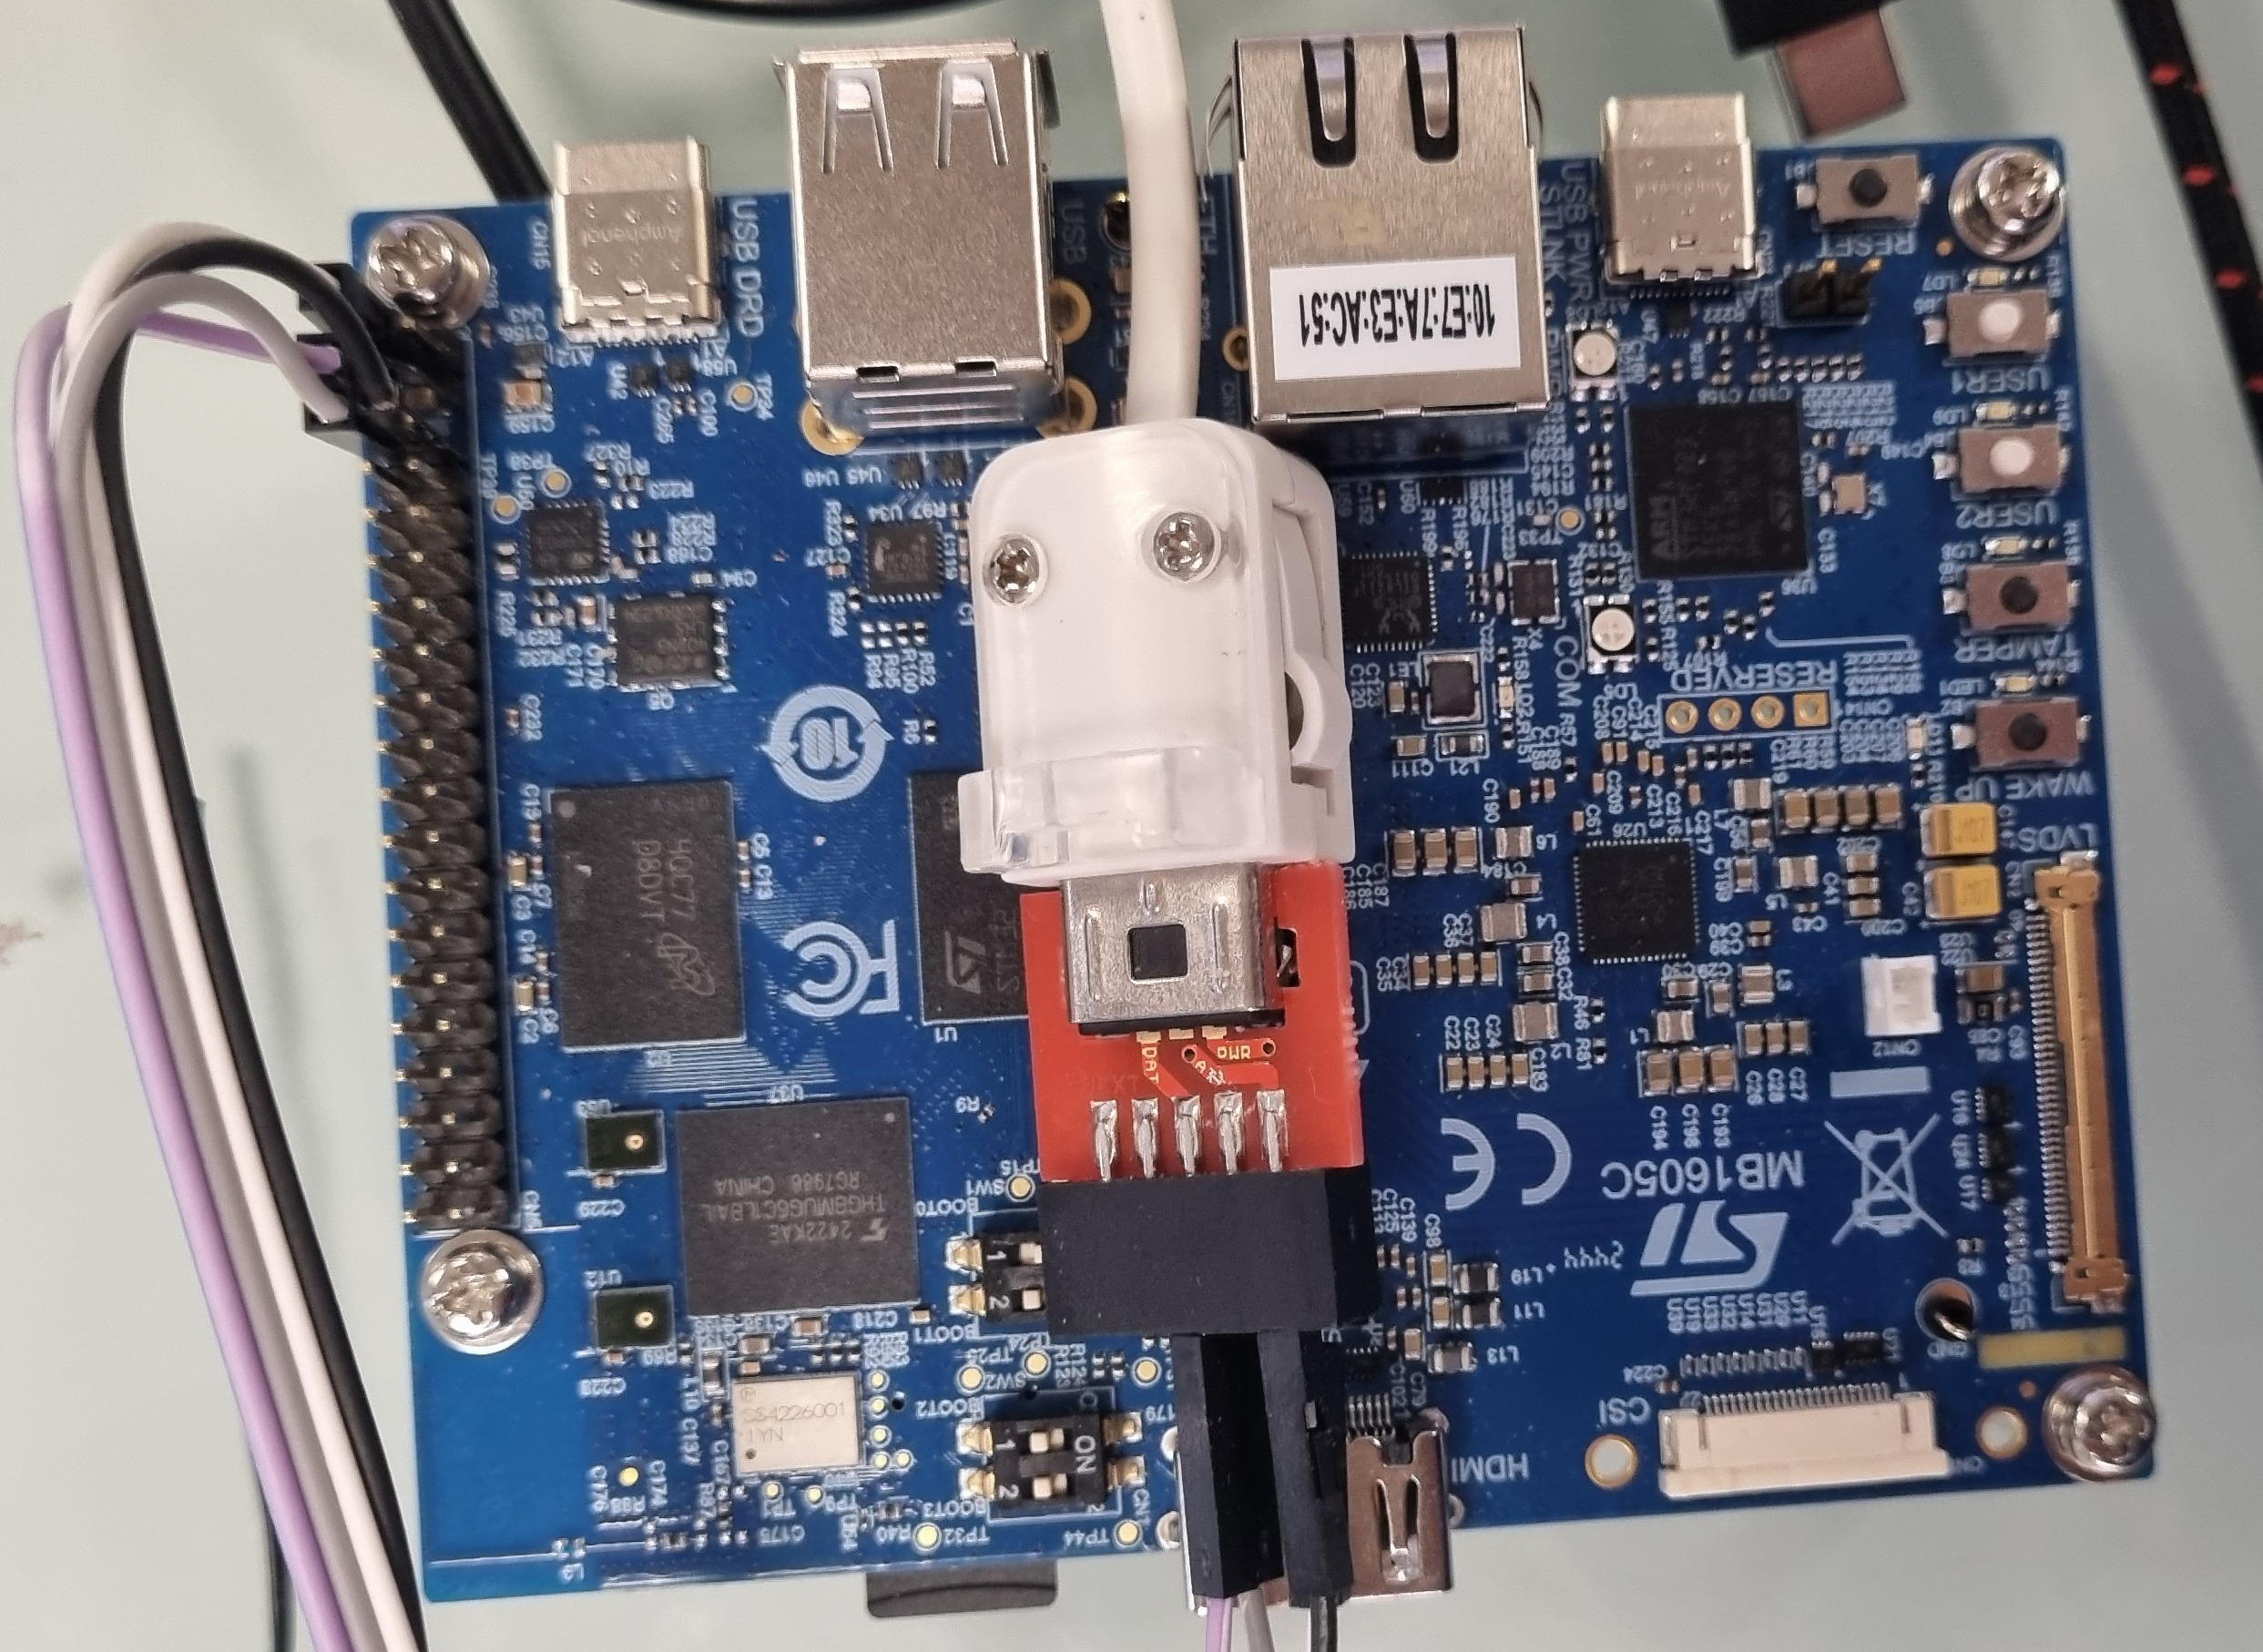
\includegraphics[width=0.7\textwidth]{common/stm32mp2_nunchuk.jpg}

In this case, most of the labels on the GPIO expansion connector correspond to the
Nunchuk pin names. Just make sure that the PWR Nunchuk pin is connected to the
3V3 GPIO expansion connector pin.

If you didn't make any mistakes, your new device should be detected at
address \code{0x52}:

\begin{bashinput}
# i2cdetect -r 1
i2cdetect: WARNING! This program can confuse your I2C bus
Continue? [y/N] y
     0  1  2  3  4  5  6  7  8  9  a  b  c  d  e  f
00:          -- -- -- -- -- -- -- -- -- -- -- -- --
10: -- -- -- -- -- -- -- -- -- -- -- -- -- -- -- --
20: -- -- -- -- -- -- -- -- -- -- -- -- -- -- -- --
30: -- -- -- -- -- -- -- -- -- -- -- -- -- -- -- --
40: -- -- -- -- -- -- -- -- -- -- -- -- -- -- -- --
50: -- -- 52 -- -- -- -- -- -- -- -- -- -- -- -- --
60: -- -- -- -- -- -- -- -- -- -- -- -- -- -- -- --
70: -- -- -- -- -- -- -- --
\end{bashinput}

We will later compile an out-of-tree kernel module to support this device.
